\begin{figure}[H]
\centering
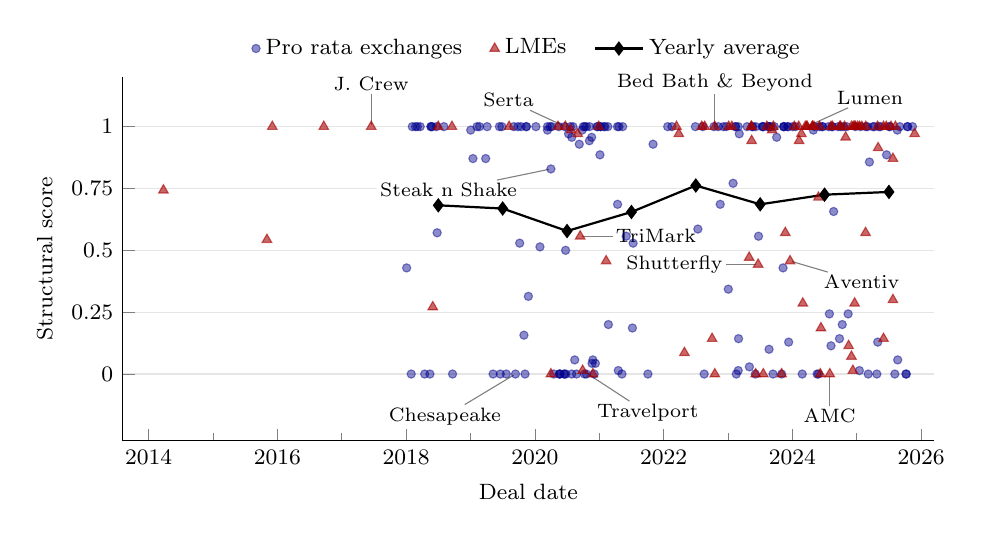
\begin{tikzpicture}
\begin{axis}[width=0.98\textwidth, height=6.2cm, xmin=2013.6, xmax=2026.2, ymin=-0.27, ymax=1.2,
  xtick={2014,2016,...,2026}, minor xtick={2015,2017,...,2025}, x tick label style={/pgf/number format/1000 sep=}, ytick={0,0.25,0.5,0.75,1},
  xlabel={Deal date}, ylabel={Structural score}, label style={font=\footnotesize}, ticklabel style={font=\footnotesize},
  ymajorgrids, grid style={gray!20}, axis lines*=left, clip=false,
  legend style={at={(0.5,1.02)}, anchor=south, draw=none, font=\footnotesize, legend columns=3, /tikz/every even column/.append style={column sep=8pt}}]
\addplot[only marks, mark=*, mark size=1.5pt, color=blue!55!black, opacity=0.45] coordinates {(2018.008,0.429) (2018.079,0.000) (2018.096,1.000) (2018.145,1.000) (2018.175,1.000) (2018.219,1.000) (2018.288,0.000) (2018.370,0.000) (2018.384,1.000) (2018.389,1.000) (2018.405,1.000) (2018.471,1.000) (2018.482,0.571) (2018.586,1.000) (2018.721,0.000) (2019.003,0.986) (2019.038,0.871) (2019.101,1.000) (2019.140,1.000) (2019.236,0.871) (2019.258,1.000) (2019.351,0.000) (2019.449,1.000) (2019.463,0.000) (2019.488,1.000) (2019.556,0.000) (2019.671,1.000) (2019.699,0.000) (2019.737,1.000) (2019.764,0.529) (2019.786,1.000) (2019.830,0.157) (2019.847,0.000) (2019.866,1.000) (2019.868,1.000) (2019.899,0.314) (2020.016,1.000) (2020.079,0.514) (2020.195,1.000) (2020.195,0.986) (2020.236,1.000) (2020.249,0.829) (2020.263,1.000) (2020.293,0.000) (2020.370,1.000) (2020.384,0.000) (2020.386,0.000) (2020.386,0.000) (2020.455,0.000) (2020.458,0.000) (2020.463,1.000) (2020.477,0.500) (2020.482,0.000) (2020.523,0.971) (2020.551,1.000) (2020.573,0.957) (2020.573,0.000) (2020.592,1.000) (2020.619,0.057) (2020.647,0.000) (2020.690,0.929) (2020.734,0.986) (2020.751,1.000) (2020.770,0.000) (2020.773,1.000) (2020.800,1.000) (2020.800,0.000) (2020.847,0.943) (2020.849,1.000) (2020.882,0.957) (2020.888,0.043) (2020.901,0.057) (2020.921,0.000) (2020.940,0.043) (2020.964,1.000) (2020.975,1.000) (2021.011,0.886) (2021.019,1.000) (2021.019,1.000) (2021.071,1.000) (2021.090,1.000) (2021.134,1.000) (2021.142,0.200) (2021.282,1.000) (2021.285,0.686) (2021.296,0.014) (2021.307,1.000) (2021.353,0.000) (2021.364,1.000) (2021.419,0.557) (2021.515,0.186) (2021.526,0.529) (2021.756,0.000) (2021.836,0.929) (2022.063,1.000) (2022.129,1.000) (2022.493,1.000) (2022.532,0.586) (2022.608,1.000) (2022.630,0.000) (2022.781,1.000) (2022.849,1.000) (2022.879,0.686) (2022.929,1.000) (2022.973,1.000) (2023.005,0.343) (2023.079,0.771) (2023.110,1.000) (2023.121,1.000) (2023.129,0.000) (2023.159,0.014) (2023.159,1.000) (2023.164,0.143) (2023.175,0.971) (2023.296,1.000) (2023.332,0.029) (2023.373,1.000) (2023.386,1.000) (2023.425,0.000) (2023.430,1.000) (2023.474,0.557) (2023.532,1.000) (2023.542,1.000) (2023.551,1.000) (2023.622,1.000) (2023.636,1.000) (2023.638,0.100) (2023.647,1.000) (2023.666,1.000) (2023.699,0.000) (2023.721,1.000) (2023.756,0.957) (2023.833,0.000) (2023.855,0.429) (2023.866,1.000) (2023.866,1.000) (2023.871,1.000) (2023.929,1.000) (2023.932,1.000) (2023.942,0.129) (2024.003,1.000) (2024.049,1.000) (2024.153,0.000) (2024.326,0.986) (2024.345,1.000) (2024.384,0.000) (2024.405,0.000) (2024.422,1.000) (2024.463,1.000) (2024.471,1.000) (2024.562,1.000) (2024.575,0.243) (2024.600,0.114) (2024.614,1.000) (2024.622,1.000) (2024.641,0.657) (2024.710,1.000) (2024.732,0.143) (2024.753,1.000) (2024.775,0.200) (2024.797,1.000) (2024.844,1.000) (2024.866,0.243) (2024.978,1.000) (2025.041,0.014) (2025.060,1.000) (2025.140,1.000) (2025.167,1.000) (2025.178,0.000) (2025.197,0.857) (2025.252,1.000) (2025.274,1.000) (2025.312,0.000) (2025.326,0.129) (2025.342,1.000) (2025.370,1.000) (2025.463,0.886) (2025.501,1.000) (2025.515,1.000) (2025.592,0.000) (2025.630,0.986) (2025.636,0.057) (2025.668,1.000) (2025.764,0.000) (2025.770,0.000) (2025.786,1.000) (2025.792,1.000) (2025.866,1.000)};
\addplot[only marks, mark=triangle*, mark size=2pt, color=red!65!black, opacity=0.6] coordinates {(2014.230,0.743) (2015.838,0.543) (2015.921,1.000) (2016.721,1.000) (2017.458,1.000) (2018.414,0.271) (2018.499,1.000) (2018.712,1.000) (2019.600,1.000) (2020.249,0.000) (2020.359,1.000) (2020.474,1.000) (2020.562,0.986) (2020.666,0.971) (2020.704,0.557) (2020.742,0.014) (2020.901,0.000) (2020.992,1.000) (2021.107,0.457) (2022.200,1.000) (2022.236,0.971) (2022.323,0.086) (2022.592,1.000) (2022.638,1.000) (2022.753,0.143) (2022.795,1.000) (2022.795,0.000) (2023.011,1.000) (2023.060,1.000) (2023.329,0.471) (2023.359,1.000) (2023.367,1.000) (2023.367,0.943) (2023.430,0.000) (2023.468,0.443) (2023.548,0.000) (2023.603,1.000) (2023.685,0.986) (2023.704,1.000) (2023.833,0.000) (2023.890,0.571) (2023.964,0.457) (2024.030,1.000) (2024.099,1.000) (2024.104,0.943) (2024.140,0.971) (2024.162,0.286) (2024.200,1.000) (2024.222,1.000) (2024.230,1.000) (2024.310,1.000) (2024.312,1.000) (2024.334,1.000) (2024.405,0.714) (2024.422,1.000) (2024.433,0.000) (2024.444,0.186) (2024.581,0.000) (2024.600,1.000) (2024.622,1.000) (2024.737,1.000) (2024.748,1.000) (2024.811,1.000) (2024.827,0.957) (2024.874,0.114) (2024.918,0.071) (2024.918,1.000) (2024.940,0.014) (2024.945,1.000) (2024.967,1.000) (2024.967,0.286) (2024.978,1.000) (2025.014,1.000) (2025.044,1.000) (2025.079,1.000) (2025.137,0.571) (2025.140,1.000) (2025.323,1.000) (2025.332,0.914) (2025.416,0.143) (2025.416,1.000) (2025.458,1.000) (2025.532,1.000) (2025.562,0.871) (2025.562,0.300) (2025.600,1.000) (2025.899,0.971)};
\addplot[black, thick, mark=diamond*, mark size=2pt] coordinates {(2018.5,0.682) (2019.5,0.669) (2020.5,0.578) (2021.5,0.655) (2022.5,0.762) (2023.5,0.686) (2024.5,0.725) (2025.5,0.736)};
\legend{Pro rata exchanges, LMEs, Yearly average}
\node[pin={[pin edge={gray, thin}, pin distance=11pt, font=\scriptsize, inner sep=1pt, fill=white, fill opacity=0.85, text opacity=1]90:J. Crew}, inner sep=0pt] at (axis cs:2017.458,1.000) {};
\node[pin={[pin edge={gray, thin}, pin distance=11pt, font=\scriptsize, inner sep=1pt, fill=white, fill opacity=0.85, text opacity=1]250:Chesapeake}, inner sep=0pt] at (axis cs:2019.699,0.000) {};
\node[pin={[pin edge={gray, thin}, pin distance=11pt, font=\scriptsize, inner sep=1pt, fill=white, fill opacity=0.85, text opacity=1]150:Serta}, inner sep=0pt] at (axis cs:2020.474,1.000) {};
\node[pin={[pin edge={gray, thin}, pin distance=11pt, font=\scriptsize, inner sep=1pt, fill=white, fill opacity=0.85, text opacity=1]200:Steak n Shake}, inner sep=0pt] at (axis cs:2020.249,0.829) {};
\node[pin={[pin edge={gray, thin}, pin distance=11pt, font=\scriptsize, inner sep=1pt, fill=white, fill opacity=0.85, text opacity=1]290:Travelport}, inner sep=0pt] at (axis cs:2020.742,0.014) {};
\node[pin={[pin edge={gray, thin}, pin distance=11pt, font=\scriptsize, inner sep=1pt, fill=white, fill opacity=0.85, text opacity=1]0:TriMark}, inner sep=0pt] at (axis cs:2020.704,0.557) {};
\node[pin={[pin edge={gray, thin}, pin distance=11pt, font=\scriptsize, inner sep=1pt, fill=white, fill opacity=0.85, text opacity=1]90:Bed Bath \& Beyond}, inner sep=0pt] at (axis cs:2022.795,1.000) {};
\node[pin={[pin edge={gray, thin}, pin distance=11pt, font=\scriptsize, inner sep=1pt, fill=white, fill opacity=0.85, text opacity=1]180:Shutterfly}, inner sep=0pt] at (axis cs:2023.468,0.443) {};
\node[pin={[pin edge={gray, thin}, pin distance=11pt, font=\scriptsize, inner sep=1pt, fill=white, fill opacity=0.85, text opacity=1]340:Aventiv}, inner sep=0pt] at (axis cs:2023.964,0.457) {};
\node[pin={[pin edge={gray, thin}, pin distance=11pt, font=\scriptsize, inner sep=1pt, fill=white, fill opacity=0.85, text opacity=1]35:Lumen}, inner sep=0pt] at (axis cs:2024.222,1.000) {};
\node[pin={[pin edge={gray, thin}, pin distance=11pt, font=\scriptsize, inner sep=1pt, fill=white, fill opacity=0.85, text opacity=1]270:AMC}, inner sep=0pt] at (axis cs:2024.581,0.000) {};
\end{axis}
\end{tikzpicture}
\caption{Where each deal falls on the structural score, by deal date}
\label{fig:spectrum}
\begin{minipage}{0.95\textwidth}\vspace{2pt}\footnotesize
\textit{Notes.} Each point is one of the 275 scored deals. 0 means every one of the 70 codings says shock and 1 means every coding says structural. The yearly average is shown for years with at least 15 deals.
\end{minipage}
\end{figure}
